\subsection{Sensor Applikation}

Bei den Komponenten der Sensor-Anwendung handelt es sich, wie in \autoref{sec:raspberrypi} erwähnt, um die beiden Bauteile:

\begin{itemize}
	\item \emph{AZDeliveryCamRasp Kamera}
	\item \emph{HC-SR501 Bewegungssensor}
\end{itemize}

\subsection{Kamera}

Bei der Kamera handelt es sich um ein eigens für den Raspberry Pi entwickeltes Modell und wird direkt an den vorhanden Kamera-Port des Raspberry Pi 3\footnote{\url{https://en.wikipedia.org/wiki/Raspberry_Pi\#/media/File:Raspberry-Pi-3-Flat-Top.jpg}} angeschlossen.

\begin{figure}[h]
	\centering
	\includegraphics[scale=0.20]{\imageDir/rpi-border-cam.jpg}
	\caption{Raspberry-Pi 3}
	\label{fig:rpi-border-cam}
\end{figure}

Anschließend muss die Kamera aktiviert werden. Dies geschieht über das, mit den meisten Linux-Distributionen mitgelieferte, Programm \emph{raspi-config\footnote{\url{https://upload.wikimedia.org/wikipedia/commons/e/ed/Raspi-config.png}}}. Dieses Programm wird auch benutzt um andere Komponenten des Raspberry Pi zu konfigurieren.

\begin{figure}[h]
	\centering
	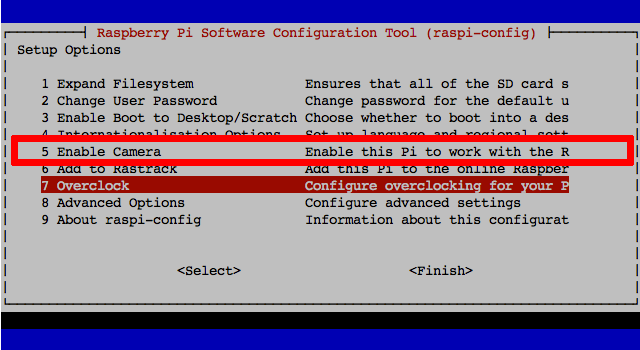
\includegraphics[scale=0.40]{\imageDir/raspi-config-cam.png}
	%By Onepiece84 (Own work) [CC BY-SA 4.0 (http://creativecommons.org/licenses/by-sa/4.0)], via Wikimedia Commons
	\caption{Raspi-config}
	\label{fig:raspi-config-cam}
\end{figure}

Zur Ansteuerung der Kamera wird das Konsolenprogramm \emph{raspistill} verwendet. Diese kann mit verschiedensten Parametern konfiguriert werden. Als Beispiel:\\
\newline
\begin{code}
	raspistill --width 1920 --height 1080 -o test.jpg\\
\end{code}
\newline
Dies erzeugt ein Bild in der Auflösung 1920 x 1080 Pixel und speichert es unter dem Dateinamen \emph{test.jpg}.

\subsection{HC-SR501 Bewegungssensor}

Der HC-SR501 Sensor wird über die GPIO-Pins des Raspberry Pi angesteuert. Hierbei werden Masse, Stromversorgung und Daten-Pin des HC-SR501 Sensors mit den GPIO-Pins verbunden. 

\begin{figure}[h]
	\centering
	\includegraphics[scale=0.20]{\imageDir/rpi-border-gpio.jpg}
	\caption{Raspberry-Pi 3}
	\label{fig:rpi-border-gpio}
\end{figure}

Die Pin-Belegung\footnote{\url{http://www.netzmafia.de/skripten/hardware/RasPi/Projekt-PIR/}} des HC-SR501

\begin{figure}[h]
	\centering
	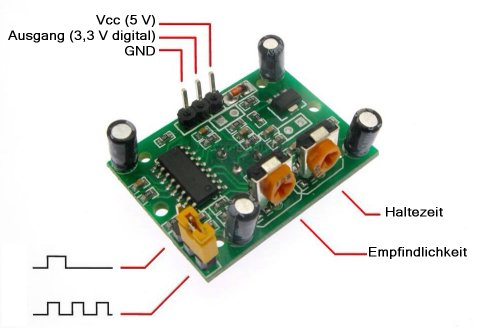
\includegraphics[scale=0.50]{\imageDir/PIR4.jpg}
	\caption{Pin-Schema HC-SR501}
	\label{fig:PIR4}
\end{figure}

ist wie folgt definiert:

\begin{itemize}
	\item Pin 1: VCC (5 Volt)
	\item Pin 2: Out, Data
	\item Pin 3: GND, Masse
\end{itemize}

zusätzlich kann die Empfindlichkeit und Haltezeit an den beiden Drehreglern eingestellt werden. Zusätzlich kann noch das Daten-Pin Verhalten über den Jumper konfiguriert werden.

\pagebreak

\subsection{GPIO}

GPIO ist die Abkürzung für General Purpose Input Output. Man bezeichnet damit programmierbare Ein- und Ausgänge für allgemeine Zwecke. Die GPIOs werden als Lötpunkt oder Pin in Form einer Stiftleiste herausgeführt und dienen als Schnittstelle zu anderen Systemen oder Schaltungen, um diese über den Raspberry Pi zu steuern. Dabei kann der Raspberry Pi bei entsprechender Programmierung digitale Signale von außen annehmen (Input) oder Signale nach außen abgeben (Output).\\

Viele der GPIOs erfüllen je nach Einstellung und Programmierung verschiedene Funktionen. Neben den typischen GPIO-Ein- und Ausgängen finden sich aber auch Pins mit der Doppelfunktion für I2C, SPI und eine serielle Schnittstelle.\\

\subsubsection{HC-SR501 GPIO Verbindung}

Für den HC-SR501 wird die Pin-Belegung wie folgt gewählt:

\begin{itemize}
	\item Pin 1: VCC (5 Volt) an Pin 2
	\item Pin 2: Out, Data an Pin 8
	\item Pin 3: GND an Pin 6
\end{itemize}

Diese Pin-Belegung erfolgt aufgrund der folgenden schematischen Darstelleung\footnote{\url{http://pi4j.com/pins/model-3b-rev1.html}}:

\begin{figure}[h]
	\centering
	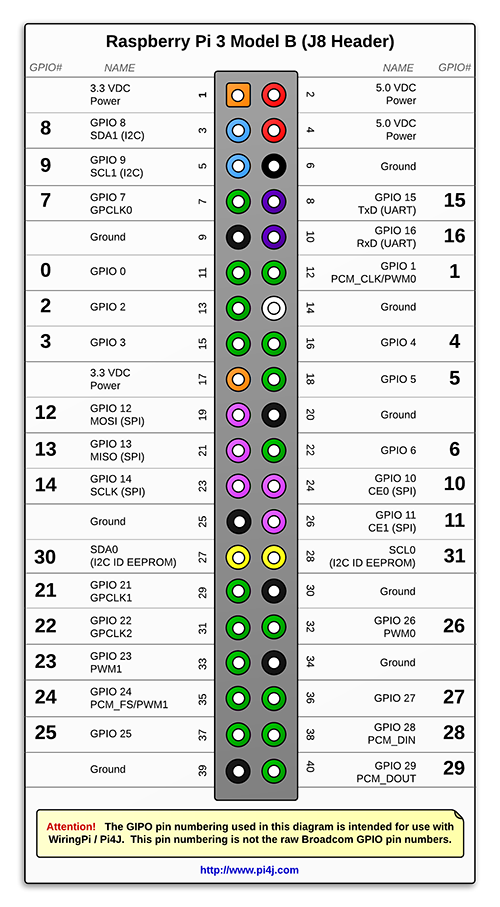
\includegraphics[scale=1.00]{\imageDir/j8header-3b.png}
	\caption{Pin-Schema}
	\label{fig:j8header-3b}
\end{figure}

\pagebreak

\subsection{Pin-Ansteuerung mit Java}

Die Ansteuerung der Pins erfolgt über die \emph{Pi4J\footnote{\url{http://pi4j.com/}}}-Bibliotheken die wiederum die \emph{WiringPi\footnote{\url{http://wiringpi.com/}}}-Bibliothek nutzt, welche die eigentliche Ansteuerung der Pins erledigt.

\subsubsection{Pi4J}
Pi4J ist eine Bibliothek  für Java, die den vollen Zugriff auf die Ressourcen des Raspberry PI ermöglicht. Mit Pi4J ist es möglich Anwendungen für Raspberry PI zu schreiben, die nur Java benötigen. Damit können praktisch alle Bibliotheken eingesetzt werden, die für Java verfügbar sind. Einschränkungen gibt es nur bei den Ressourcen des Raspberry.

\subsubsection{WiringPi}
WiringPi ist ein nützliches Framework um die GPIO Ein-und Ausgänge am Raspberry Pi zu schalten. Das Ziel dieser Bibliothek ist es, eine einzige gemeinsame Plattform und Programmierschnistelle für den Zugriff auf die GPIOs des Rapsberry Pi für verschiedene Programmiersprachen zur Verfügung zu stellen. Im Kern ist WiringPi eine C-Bibliothek, aber sie steht auch in Ruby und Python zur Verfügung.

\begin{code}
	\caption{gpio-controller.java}
	\yamlFile{\srcDir/gpio-controller.java}
	\label{src:gpio-controller}
\end{code}